% !TEX TS-program = pdflatex
% !TEX encoding = UTF-8 Unicode

% This is a simple template for a LaTeX document using the "article" class.
% See "book", "report", "letter" for other types of document.

\documentclass[11pt]{article} % use larger type; default would be 10pt

\usepackage[utf8]{inputenc} % set input encoding (not needed with XeLaTeX)

%%% Examples of Article customizations
% These packages are optional, depending whether you want the features they provide.
% See the LaTeX Companion or other references for full information.

%%% PAGE DIMENSIONS
\usepackage{geometry} % to change the page dimensions
\geometry{a4paper} % or letterpaper (US) or a5paper or....
% \geometry{margin=2in} % for example, change the margins to 2 inches all round
% \geometry{landscape} % set up the page for landscape
%   read geometry.pdf for detailed page layout information

\usepackage{graphicx} % support the \includegraphics command and options

% \usepackage[parfill]{parskip} % Activate to begin paragraphs with an empty line rather than an indent

%%% PACKAGES
\usepackage{booktabs} % for much better looking tables
\usepackage{array} % for better arrays (eg matrices) in maths
\usepackage{paralist} % very flexible & customisable lists (eg. enumerate/itemize, etc.)
\usepackage{verbatim} % adds environment for commenting out blocks of text & for better verbatim
\usepackage{subfig} % make it possible to include more than one captioned figure/table in a single float
% These packages are all incorporated in the memoir class to one degree or another...

%%% HEADERS & FOOTERS
\usepackage{fancyhdr} % This should be set AFTER setting up the page geometry
\pagestyle{fancy} % options: empty , plain , fancy
\renewcommand{\headrulewidth}{0pt} % customise the layout...
\lhead{}\chead{}\rhead{}
\lfoot{}\cfoot{\thepage}\rfoot{}

%%% SECTION TITLE APPEARANCE
\usepackage{sectsty}
\allsectionsfont{\sffamily\mdseries\upshape} % (See the fntguide.pdf for font help)
% (This matches ConTeXt defaults)

%%% ToC (table of contents) APPEARANCE
\usepackage[nottoc,notlof,notlot]{tocbibind} % Put the bibliography in the ToC
\usepackage[titles,subfigure]{tocloft} % Alter the style of the Table of Contents
\renewcommand{\cftsecfont}{\rmfamily\mdseries\upshape}
\renewcommand{\cftsecpagefont}{\rmfamily\mdseries\upshape} % No bold!

%%% END Article customizations

%%% The "real" document content comes below...

\title{EECS 233 HW1}
\author{Benjamin Pierce (bgp12)}
\date{9/4/17} % Activate to display a given date or no date (if empty),
         % otherwise the current date is printed 

\begin{document}
\maketitle

\section{Questions}



\subsection{Question 1}
\subsubsection{Run Time Less Then 1s}

\begin{center}
Fig. 1.1.1: Algorithim 1
\begin{tabular} { |c|c| }
\hline
N = 0&Time Elapsed: 0ms\\
N = 10000000&Time Elapsed: 6ms\\
N = 20000000&Time Elapsed: 7ms\\
N = 30000000&Time Elapsed: 11ms\\
N = 40000000&Time Elapsed: 14ms\\
N = 50000000&Time Elapsed: 15ms\\
N = 60000000&Time Elapsed: 20ms\\
\hline
\end{tabular}
\end{center}

\begin{center}
Fig. 1.1.2: Algorithm 2
\begin{tabular} { |c|c| }
\hline
N = 0      & Time Elapsed: 0ms \\
N = 1000 & Time Elapsed: 3ms \\
N = 2000 & Time Elapsed: 3ms \\
N = 3000 & Time Elapsed: 3ms \\
N = 4000 & Time Elapsed: 7ms \\
N = 5000 & Time Elapsed: 9ms \\
N = 6000 & Time Elapsed: 12ms \\
\hline
\end{tabular}
\end{center}

\begin{center}
Fig. 1.1.3: Algorithm 3
\begin{tabular} { |c|c| }
\hline
N = 0&Time Elapsed: 0ms \\
N = 1000&Time Elapsed: 3ms \\
N = 2000&Time Elapsed: 2ms \\
N = 3000&Time Elapsed: 3ms \\ 
N = 4000&Time Elapsed: 5ms \\ 
N = 5000&Time Elapsed: 7ms \\
N = 6000&Time Elapsed: 12ms \\
\hline
\end{tabular}
\end{center}
\par

\subsubsection{Run Time Greater then 1s}
\begin{center}
Fig. 1.2.1: Algorithim 1
\begin{tabular} { |c|c| }
\hline
N = 0&Time Elapsed: 0ms \\
N = 10000000000&Time Elapsed: 3194ms \\
N = 20000000000&Time Elapsed: 6440ms \\
N = 30000000000&Time Elapsed: 9418ms \\
N = 40000000000&Time Elapsed: 12536ms \\
N = 50000000000&Time Elapsed: 15291ms \\
N = 60000000000&Time Elapsed: 18557ms \\
\hline
\end{tabular}
\end{center}

\begin{center}
Fig. 1.2.2: Algorithim 2
\begin{tabular} { |c|c| }
\hline
N = 0&Time Elapsed: 0ms     \\
N = 100000&Time Elapsed: 4098ms \\
N = 200000&Time Elapsed: 17206ms \\ 
N = 300000&Time Elapsed: 27928ms \\
N = 400000&Time Elapsed: 51137ms \\ 
N = 500000&Time Elapsed: 80322ms \\
N = 600000&Time Elapsed: 118394ms \\
\hline
\end{tabular}
\end{center}

\begin{center}
Fig 1.2.3: Algorithm 3
\begin{tabular} { |c|c| }
\hline
N = 0&Time Elapsed: 0ms \\
N = 100000&Time Elapsed: 4098ms \\
N = 200000&Time Elapsed: 18293ms \\
N = 300000&Time Elapsed: 29799ms \\
N = 400000&Time Elapsed: 54061ms \\
N = 500000&Time Elapsed: 80339ms \\
N = 600000&Time Elapsed: 111339ms \\
\hline
\end{tabular}
\end{center}
\par

\subsection{Question 2}


\subsubsection{Run Time Less Then 1s}
\includegraphics{under1K}

Blue:Algorithm 1; Red:Algorithm 2; Green:Algorithm 3

\subsubsection{Run Time Greater Then 1s}
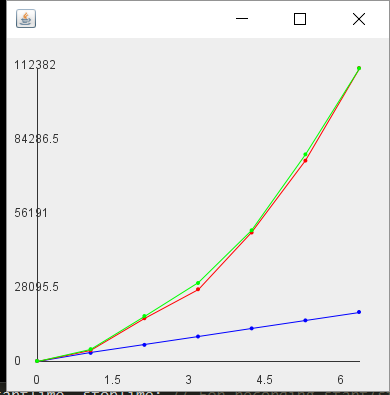
\includegraphics{Over1K}

Blue:Algorithm 1; Red:Algorithm 2; Green:Algorithm 3

\subsection{Question 3}
The results appear to be roughly as expected. The first algorithm executes a single \textit{for} loop, as as such run in $O(n)$ time. The second algorithm executes nested \textit{for} loops; therefore, it runs in $O(n^2)$ time. The third algorithm executes a single \textit{for} loop, and then a nested loop, giving it a designation of $O(n^2)$. In the results, the first algorithm increases linearly for increasing \textit{n}, as expected with an $O(n)$ algorithm. The second algorithm appears to increase quadratically as expected. The third algorithim also increases quadratically, with slight interference at small \textit{n} from the initial \textit{for} loop. 

\subsection{Question 4}
In the first algorithm, there is little diffrence for large or small \textit{n}, due to the algorithm's linearity. Likewise, the second algorithm behaves as it did with small \textit{n}. However, the third algorithm shows a different result; as \textit{n} increases, the graph becomes more quadratic. This is because of the dominance of the polynomial term $n^2$ as the \textit{n} time delay caused by the first \textit{for} loop becomes less important as the \textit{$n^2$} term become far larger. Run times longer then one second can have multiple uses, such as in in paralell processing when it becomes important that two cores operate in tandem; in the case that a core falls behind, the other must take extra time so that it does not attempt to process data that doesn't exist. 



\end{document}


